\documentclass[tikz,border=15pt]{standalone}
\usepackage{amsmath,amssymb}

\begin{document}
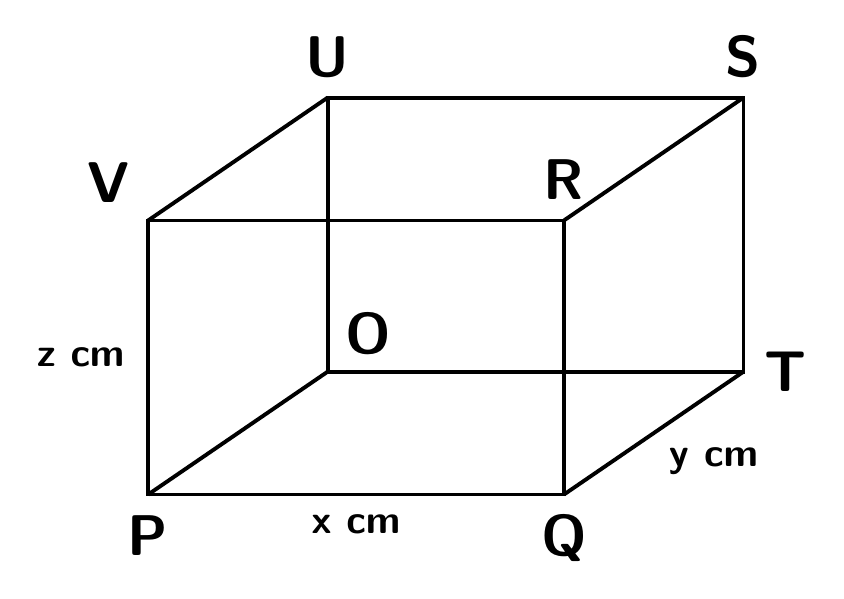
\begin{tikzpicture}[scale=1.2]
    % Front face coordinates: P(0,0), Q(4.4,0), R(4.4, 2.9), V(0, 2.9)
    \coordinate (P) at (0, 0);
    \coordinate (Q) at (4.4, 0);
    \coordinate (R) at (4.4, 2.9);
    \coordinate (V) at (0, 2.9);
    
    % Oblique depth offset: dx = 1.9, dy = 1.3
    \coordinate (O) at (1.9, 1.3);
    \coordinate (T) at (6.3, 1.3);
    \coordinate (S) at (6.3, 4.2);
    \coordinate (U) at (1.9, 4.2);
    
    % Draw front face
    \draw[line width=1.4pt] (P) -- (Q) -- (R) -- (V) -- cycle;
    
    % Draw back face
    \draw[line width=1.4pt] (O) -- (T) -- (S) -- (U) -- cycle;
    
    % Draw connecting depth edges
    \draw[line width=1.4pt] (P) -- (O);
    \draw[line width=1.4pt] (Q) -- (T);
    \draw[line width=1.4pt] (R) -- (S);
    \draw[line width=1.4pt] (V) -- (U);
    
    % Vertices labels in bold sans-serif
    \node[below=4pt, font=\huge\sffamily\bfseries] at (P) {P};
    \node[below=4pt, font=\huge\sffamily\bfseries] at (Q) {Q};
    \node[above=4pt, font=\huge\sffamily\bfseries] at (R) {R};
    \node[above left=3pt, font=\huge\sffamily\bfseries] at (V) {V};
    
    \node[above right=3pt, font=\huge\sffamily\bfseries] at (O) {O};
    \node[right=4pt, font=\huge\sffamily\bfseries] at (T) {T};
    \node[above=4pt, font=\huge\sffamily\bfseries] at (S) {S};
    \node[above=4pt, font=\huge\sffamily\bfseries] at (U) {U};
    
    % Dimensions in clean bold font
    \node[below=4pt, font=\Large\sffamily\bfseries] at (2.2, 0) {\textit{x} cm};
    \node[below right=2pt, font=\Large\sffamily\bfseries] at (5.35, 0.65) {\textit{y} cm};
    \node[left=5pt, font=\Large\sffamily\bfseries] at (0, 1.45) {\textit{z} cm};
    
\end{tikzpicture}
\end{document}
